
\section{Installation and Getting Started}
\label{sec:install_start}

This section should help you to do the first step with the CLIB
library. If you can read this documentation from your own
distribution, you probably can skip it\ldots

\subsection{Installation}
\label{sec:install_start:install}

Installation of the CLIB library should be a very simple step. Once
you have obtained the distribution file \texttt{CLIB.tgz}, you just
need to unpack the distribution, using either GNU \texttt{tar} or the
combination of \texttt{gzip} and a conventional UNIX
\texttt{tar}. This will create a subdirectory named \texttt{CLIB} in
the current directory. To install CLIB now just type 

\begin{verbatim}
cd CLIB
make install
\end{verbatim}
and the library should install itself. If you do not have a recent
version of the GCC compiler, you may need to edit
\texttt{CLIB/Makefile.vars} to select a different compiler and linker, and
to select appropriate options. You may also want to edit this file if
you have a non-standard system and lack the utilities necessary for
the normal building of the library.

The default installation procedure will not build the documentation,
as local \LaTeX{} setups seem to differ a lot between sites. To
build the documentation, you need \LaTeX2e{}. If your local \LaTeX2e{}
executable is named \texttt{latex}, just use

\begin{verbatim}
make documentation
\end{verbatim}
in the \texttt{CLIB} directory to typeset the documentation.
Otherwise, edit the file \texttt{CLIB/Makefile.vars} to point to your
\LaTeX2e{} executable (or \texttt{cd} to \texttt{CLIB/DOC/} and run
\LaTeX2e{} on \texttt{clib.tex} and \texttt{eprover.tex} manually).

\subsection{Getting Started}
\label{sec:install_start:start}

Once you managed to install the library, you may want to look around
and see what is offered. Fig~\ref{fig:install_start:start:structure}
shows the basic layout of the directory structure of CLIB.


\begin{figure}[htb]
  \begin{center}
    \mbox{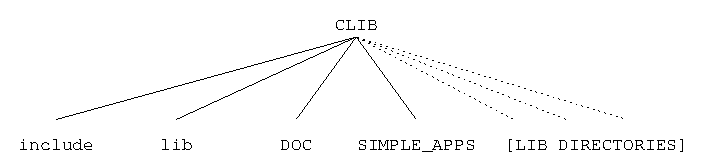
\epsfig{file=file_layout.eps}} % Export with 80%
    \caption{Directory structure of CLIB}
    \label{fig:install_start:start:structure}
  \end{center}
\end{figure}

If the documentation were anywhere close to complete, the \texttt{DOC}
directory would be the most important one for each new user. Even
though this is not yet the case, it should pay to check this directory
and read whatever rudimentary documentation can be found in the file
\texttt{clib.dvi}\footnote{As this text is contained in the CLIB
  documentation, you probably already are reading it\ldots}.

Other important directories are the \texttt{include} directory, which
should contain links to all header files provided by the library, and
the \texttt{lib} directory, which contains the individual library
parts. 

If you want to make use of this library for you own project, the
\texttt{SIMPLE\_APPS} directory has some simple examples that
illustrate the use of the library.

If you change part of the library, and want to remake all modules
depending on your changes, issuing

\begin{verbatim}
make top
\end{verbatim}
in any of the CLIB subdirectories will recompile all parts of the
libraries (more exactly, it will remake all code in directories
specified in the top level \texttt{Makefile} variable
\texttt{CODE}). A simple 

\begin{verbatim}
make
\end{verbatim}
will just remake all parts in the current directory.


\subsection{Conventions used in the Manual}
\label{sec:install_start:conventions}

Each important subsection of the library is first discussed in general
terms, sometimes including the most important data structures. After
that, the relevant functions of the calling interface are described,
giving first the function prototype and then a short description of
the function. Some functionality is implemented by C preprocessor
macros. Such macros are described as though they were functions, but
the prototype given is preceded by \texttt{MACRO}, and arguments may
be given without a type if the macro in question is defined for
multiple types.


%%% Local Variables: 
%%% mode: latex
%%% TeX-master: "clib"
%%% End: 
